\section{Neural Networks and Deep Learning \problemworth{20}}

In the following set of questions, we will discuss feed-forward and backpropagation for neural networks.

We will consider two kinds of hidden nodes/units for our neural network. The first cell (Cell A) operates as a weighted sum with no activation function. Given a set of input nodes and their weights, it outputs the weighted sum. The second cell (Cell B) operates as a power function. It takes only one input along with the weight and outputs the power of input to the weight as the output. We provide illustrations for both the nodes in Figure~\ref{fig:nn-nodes}. Note that $\mathbf{x} = [x_1, x_2, \dots, x_n]^T$ and $\mathbf{w} = [w_1, w_2, \dots, w_n]^T$.

\begin{figure}[h]
\centering
\begin{subfigure}{.5\textwidth}
  \centering
  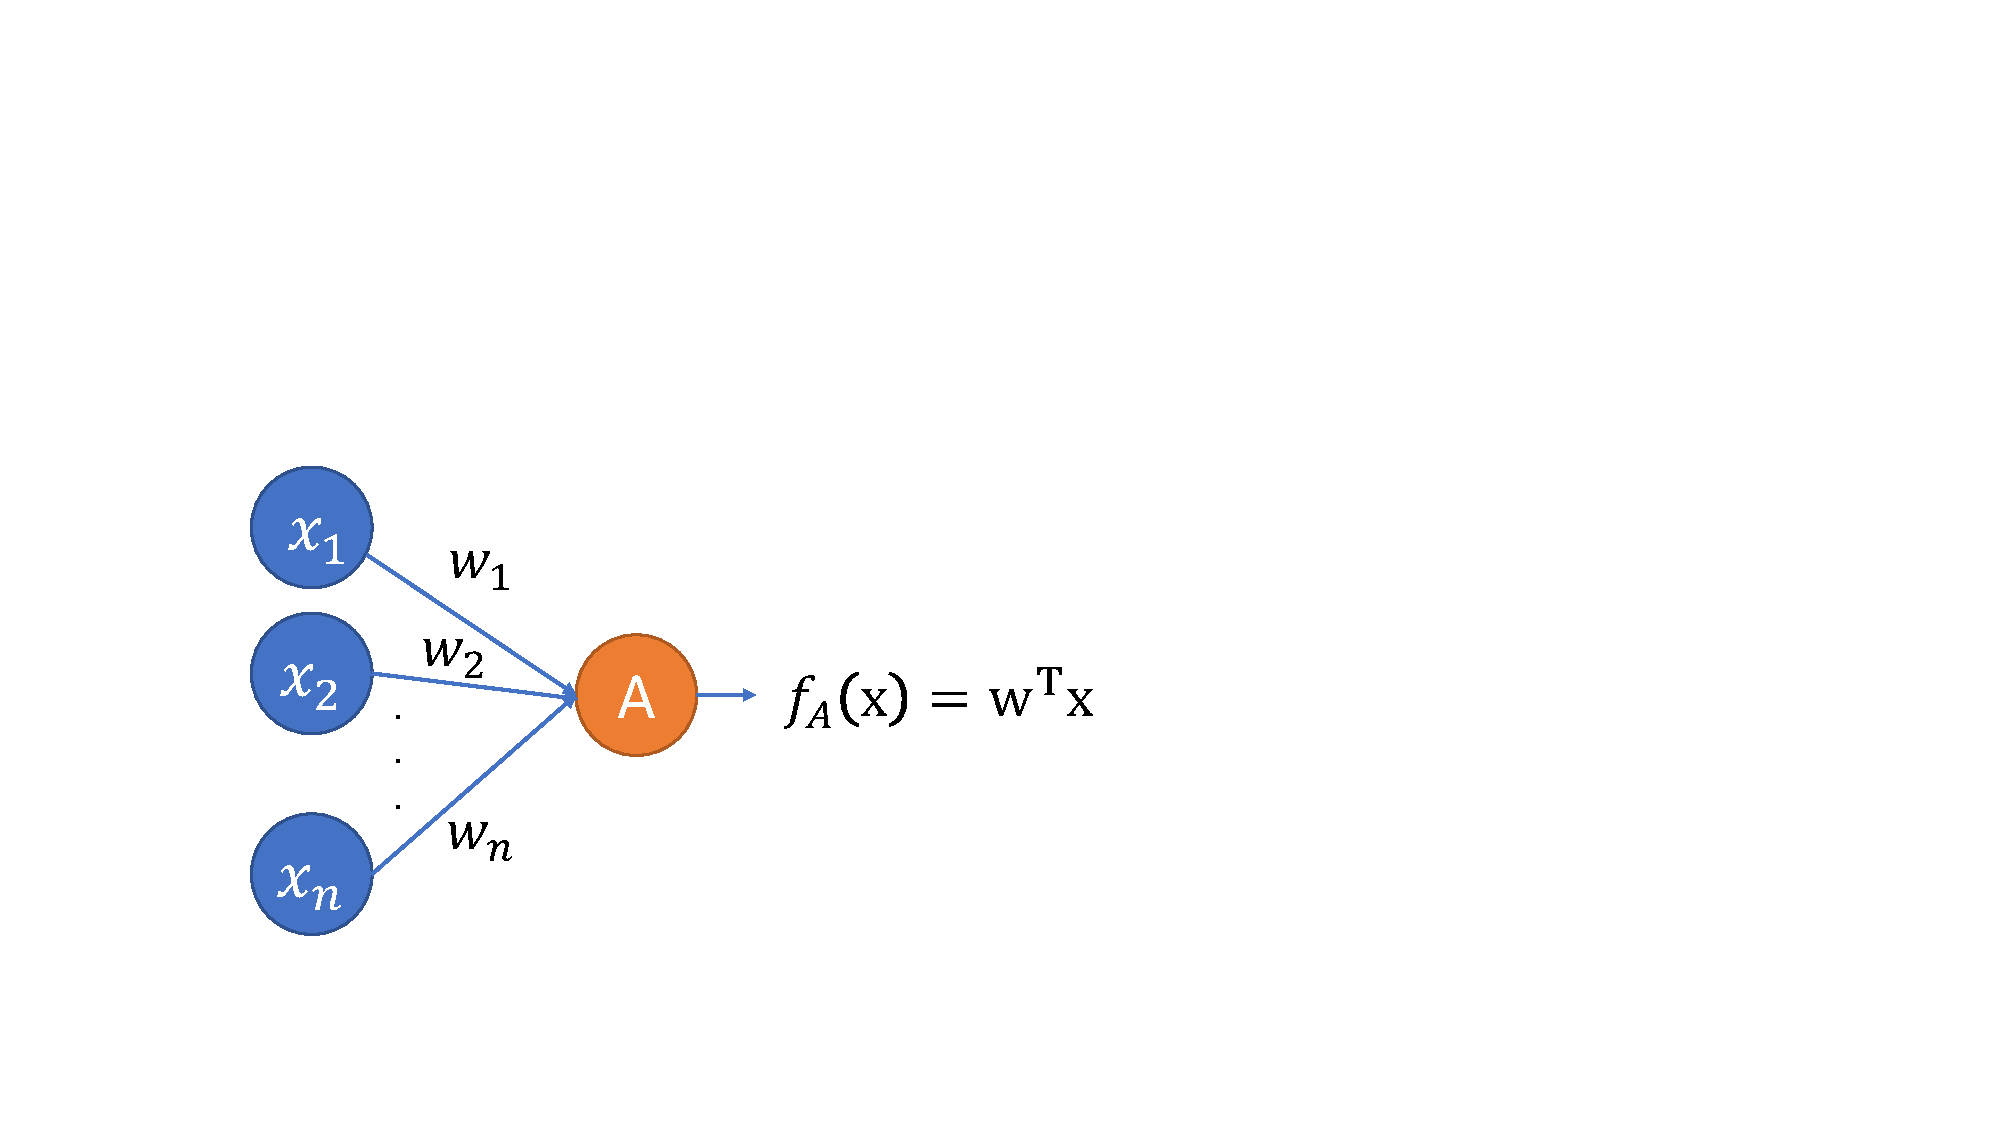
\includegraphics[width=.8\linewidth]{hw2-images/cell-a.pdf}
  \caption{}
  \label{fig:sub1}
\end{subfigure}%
\begin{subfigure}{.5\textwidth}
  \centering
  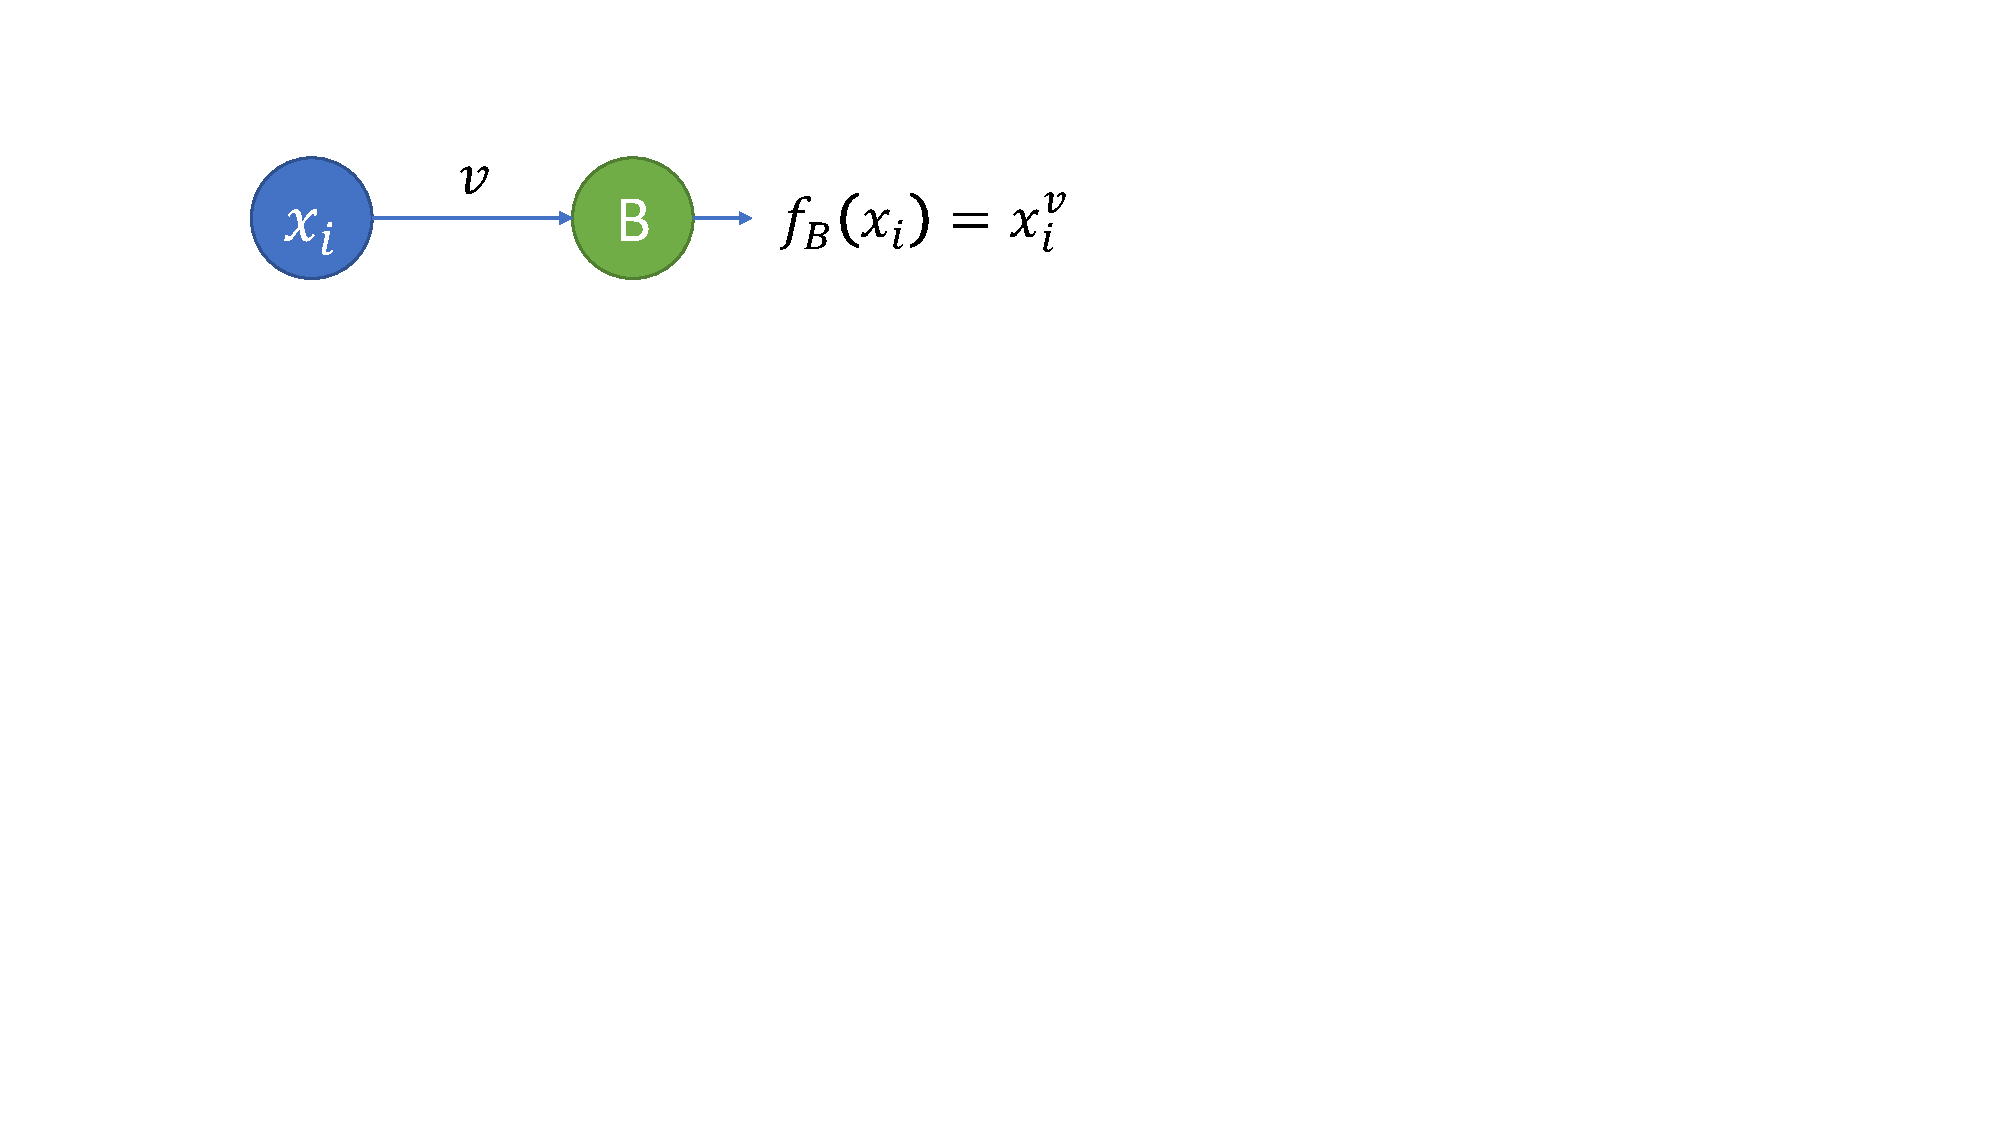
\includegraphics[width=.8\linewidth]{hw2-images/cell-b.pdf}
  \caption{}
  \label{fig:sub2}
\end{subfigure}
\caption{An illustration of Cell A and Cell B used in the neural network. (a) On the left, we have Cell A - Weighted sum. It simply computes the weighted sum over the input nodes. (b) On the right, we have Cell B - It computes power of the input node over the weight}
\label{fig:nn-nodes}
\end{figure}

Using these two kinds of hidden nodes, we build a two-layer neural network as shown in Figure~\ref{fig:nn-network}. The inputs to the neural network is $\mathbf{x} = [x_1, x_2, x_3]^T$ and the output is $\hat{y}$. The parameters of the model are $\mathbf{v} = [v_1, v_2, v_3]^T$ and $\mathbf{w} = [w_1, w_2, w_3]^T$.

\begin{figure}[h]
    \centering
    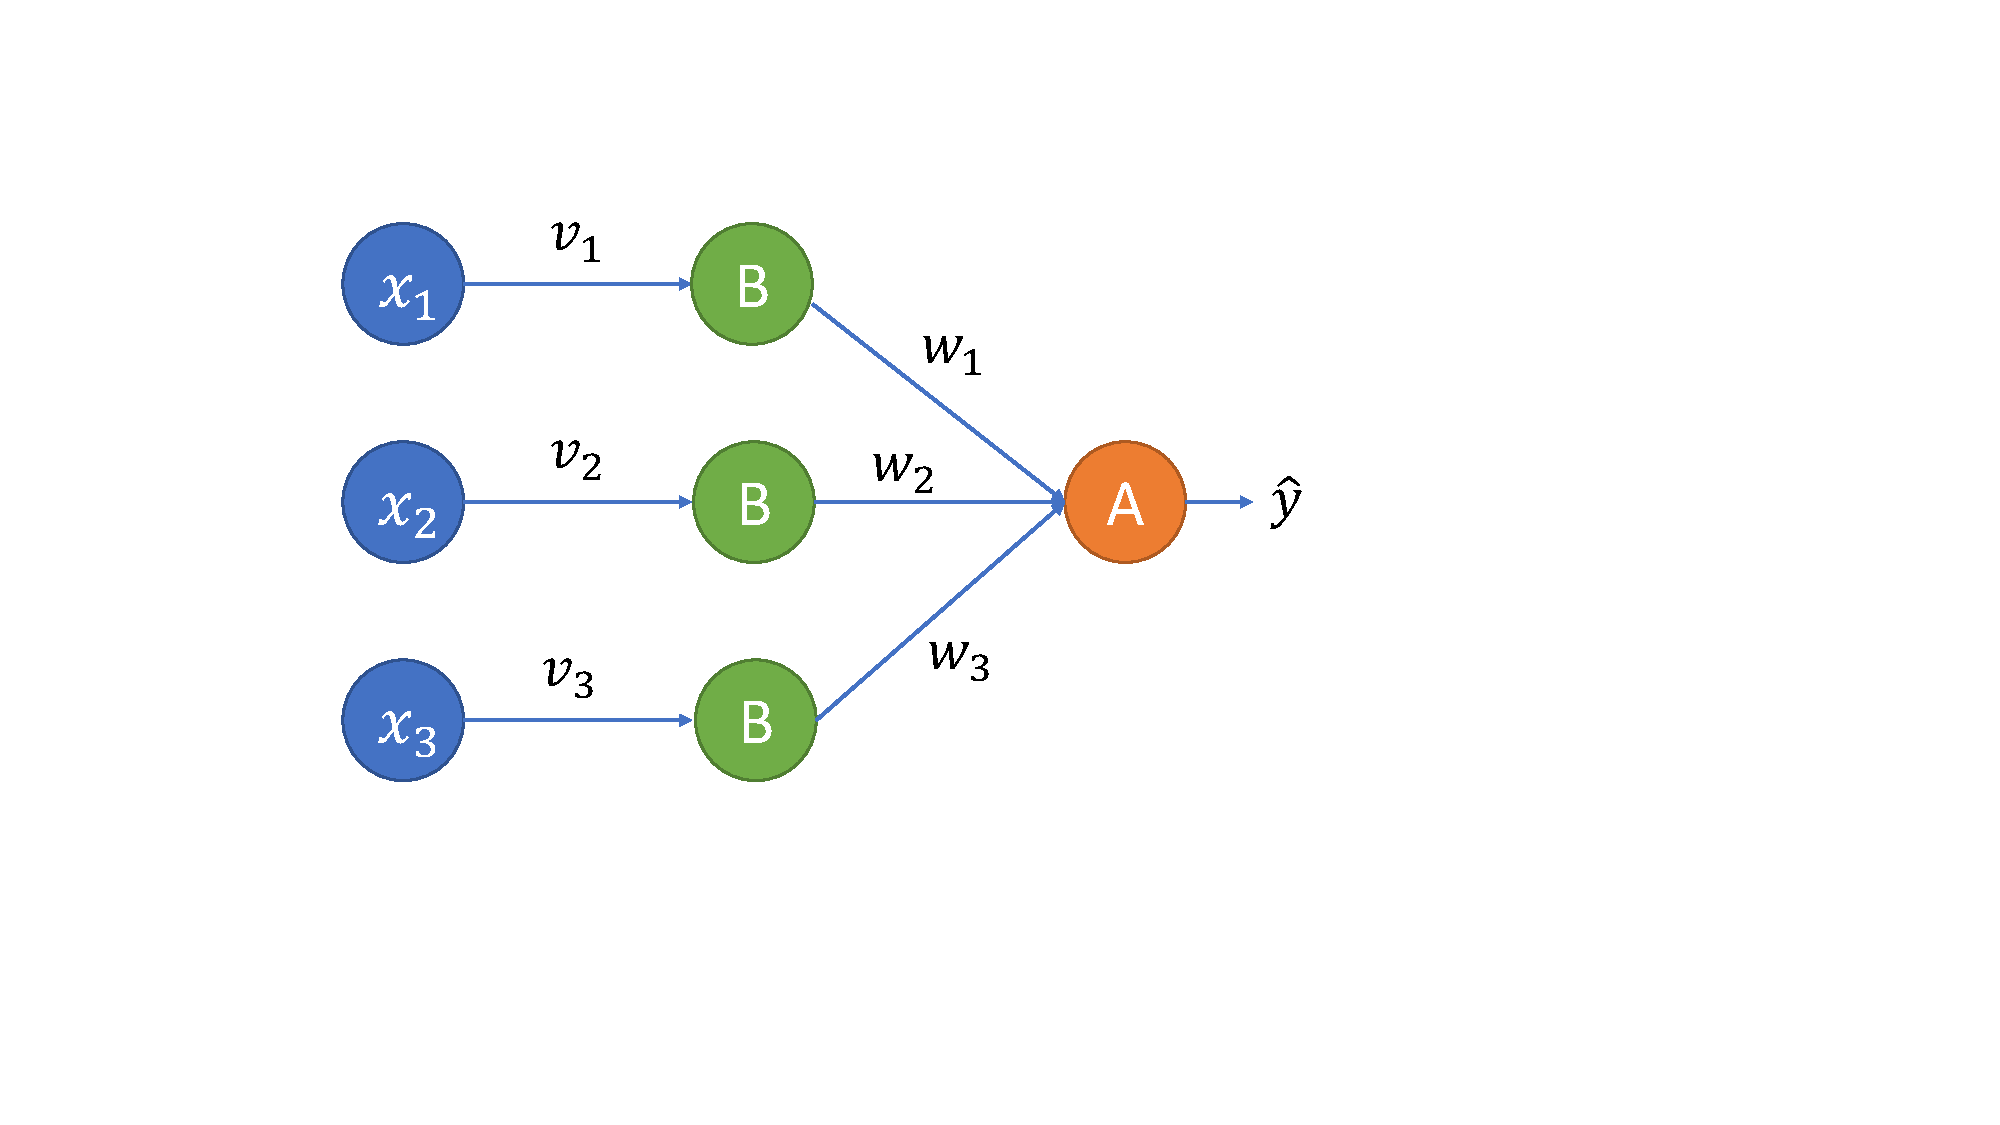
\includegraphics[width=.5\linewidth]{hw2-images/neural-network.pdf}
    \caption{Architecture of the neural network.}
    \label{fig:nn-network}
\end{figure}

\begin{enumerate}
    \item \itemworth{4}
    We would like to compute the feed-forward for the network. Mathematically, compute the expression for $\hat{y}$ given the neural network in terms of $\mathbf{x}, \mathbf{v}, \mathbf{w}$.
    
    \solution{
      \[
        \hat{y} = w_1(x_1^{v_1}) + w_2(x_2^{v_2})+w_3(x_3^{v_3})
      \]
    }
    
    \item \itemworth{2}
    Utilizing the expression for $\hat{y}$ computed in (a), compute the predicted value $\hat{y}$ when $\mathbf{x} = [1,3,2]^T, \mathbf{v}=[1,0,2]^T, \mathbf{w}=[-4,3,1]^T$

    \solution{
      \[
        \hat{y} = -4(1) + 3(1) + 1(4) = 3
      \]
    }
    
    
\end{enumerate}

We want to now utilize the backpropagation algorithm to update the weights of this neural network. First we will compute the gradients with respect to the weights. For the following parts, we are only interested in updating $v_1$ and $w_1$ in the network.

\begin{enumerate}
    \setcounter{enumi}{2}
    \item \itemworth{5} Let's derive the expression for gradients for the weights. More specifically, compute the expressions for $\frac{\partial \hat{y}}{\partial w_1}$ and $\frac{\partial \hat{y}}{\partial v_1}$. Using the values described in part (b), compute the final values of these expressions. (\textbf{Hint:} Use the expression computed in part (a))
    
    \solution{
      \begin{gather*}
        \frac{\partial \hat{y}}{\partial w_1} = x_1^{v_1} = 1 \\
        \frac{\partial \hat{y}}{\partial v_1} = w_1(x_1^{v_1}ln(x_1)) = 0 \\
      \end{gather*}
    }
    
    
    \item \itemworth{3} Assuming the loss function is $\mathcal{L} = (y - \hat{y})^2$ where $y$ is the true value of the output and $\hat{y}$ is the predicted output from the neural network. Compute the expression for  $\frac{\partial \mathcal{L}}{\partial \hat{y}}$. Let the actual value of $y = 5$. What will the value for this expression be?
    
    \solution{
      \begin{equation*}
        \begin{split}
          \frac{\partial L}{\partial \hat{y}} & = -2(y - \hat{y}) \\
          & = -2(5 - 3) = -4
        \end{split}
      \end{equation*}
    }
    
    \item \itemworth{3} Using parts (c) and (d), compute the values for the expressions for $\frac{\partial \mathcal{L}}{\partial v_1}$ and $\frac{\partial \mathcal{L}}{\partial w_1}$. (\textbf{Hint:} Use the chain rule)
    
    \solution{
      \begin{gather*}
        \frac{\partial L}{\partial v_1} = \frac{\partial L}{\partial \hat{y}} \frac{\partial \hat{y}}{\partial v_1} = -4(0) = 0 \\
        \frac{\partial L}{\partial w_1} = \frac{\partial L}{\partial \hat{y}} \frac{\partial \hat{y}}{\partial w_1} = -4(1) = -4
      \end{gather*}
    }

\end{enumerate}

We will finally use the gradient descent algorithm to update the weights for $v_1$ and $w_1$. Note that the gradient descent update formula for a parameter $w$ is given as $w \leftarrow w - \eta \frac{\partial \mathcal{L}}{\partial w}$. Assume the learning rate $\eta = 1$ for the following question.

\begin{enumerate}
    \setcounter{enumi}{5}
    \item \itemworth{3} Using the gradient descent update rule explained above, compute the updated values for $v_1$ and $w_1$.
    
    \solution{
      \begin{align*}
        w_1 &\leftarrow -4 - 1(-4) & v_1 &\leftarrow 1 - 1(0) \\
        w_1 &\leftarrow 0 & v_1 &\leftarrow 1
      \end{align*}
    }
    
\end{enumerate}